\section{Dependence of ion velocity direction on altitude (AB 5.2)}
We look back at the result from previous, where we found an expression for the ion and electron velocity given on the form as in \cref{eq:L12_v_i_equation_big}.

We now neglect all other forces except the electrostatic field \(\gf{E}\) for a while and assume \(\gf{E}\cdot\gf{B}=0\). \Cref{eq:L12_v_i_equation_big} will then look like
\begin{equation*}
    \gf{v}_i=\frac{k_i}{1+k_i^2}\frac{\gf{E}_\perp}{B}+\frac{k_i^2}{1+k_i^2}\frac{\gf{E}_\perp\times\gf{B}}{B^2}
\end{equation*}
with a change of sign on the first term giving the same equation for electrons.

In the F-region we have that \(\nu_{in}\ll\Omega_i\Rightarrow k_i\gg 1\) which then imply
\begin{equation*}
    \gf{v}_i\approx\frac{\gf{E}_\perp\times\gf{B}}{B^2}
\end{equation*}
i.e.\ the ions \(\gf{E}\times\gf{B}\) drift.

In the D-region the opposite is the case, \(\nu_{in}\gg\Omega_i\Rightarrow k_i\ll 1\) which imply
\begin{equation*}
    \gf{v}_i\approx k_i\frac{\gf{E}_\perp}{B}
\end{equation*}
We introduce an angle \(\theta_i\) to denote the angle between the electric field and the ion velocity. This will be given as
\begin{equation*}
    \theta_i=k_i=\frac{\Omega_i}{\nu_i}
\end{equation*}
Therefore, in the F-region we have \(\theta_{i,\tn{F-region}}=\SI{90}{\degree}\), at 125 km altitude where the collision frequency is about the same as the gyro frequency we have \(\theta_{i,\tn{125 km}}=\SI{45}{\degree}\) and in the D-region we have \(\theta_{i,\tn{D-region}}=\SI{0}{\degree}\). As we can observe ion velocities in the ionosphere by incoherent scatter radar experiments, we can derive at different heights the angle between the electric field and the ion velocity. If this angle does not agree with the angle \(\theta_i\) derived above, we can infer that there must have been a neutral wind present.

The magnitude of the ion velocity is
\begin{equation*}
    v_i=k_i{\left(1+k_i^2\right)}^{-1/2}\frac{E}{B}=\sin\theta_i\frac{E}{B}
\end{equation*}
From this we see that in the D-region the ion velocity goes to zero (\(\theta_i\approx\SI{0}{\degree}\)) due to the high number of collisions. In the F-region, upper ionosphere, where \(\theta_i\approx\SI{90}{\degree}\) we get that \(v_i\approx E/B\).

The same can be done for electrons, and it can be shown that
\begin{equation*}
    \tan\theta_e=-k_e=-\frac{\Omega_e}{\nu_{en}}
\end{equation*}
with a magnitude of
\begin{equation*}
    v_e=k_e{\left(1+k_e^2\right)}^{-1/2}\frac{E}{B}=-\sin\theta_e\frac{E}{B}
\end{equation*}
The different directions of the velocities at different heights is illustrated in \cref{fig:L14_v_i_v_e_electric_field}.
\begin{figure}[t]
    \centering
    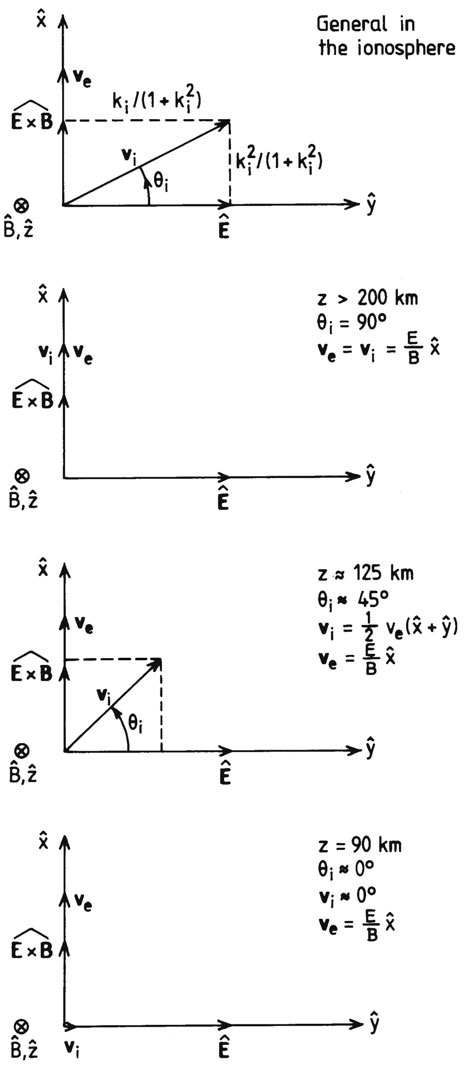
\includegraphics[width=.4\linewidth]{bilder/L14_v_i_v_e_electric_field.jpg}
    \caption{Vector diagrams showing the variation of vi and ve in the applied electric field for three different altitudes in the ionosphere.}\label{fig:L14_v_i_v_e_electric_field}
\end{figure}
The rotation of the ion velocity with respect to the electric field and the electron velocity in the ionosphere is, as we have demonstrated above, a result of varying collision frequency with height.

\section{Current density in the ionosphere}
We write out the current with the expressions for \(\gf{v}_i\) and \(\gf{v}_e\) we found in \cref{eq:L12_v_i_equation_big}. This yields
\begin{align}
    \gf{j}&=n_{e}e\left \{\left(\frac{k_e}{1+k_e^2}+\frac{k_i}{1+k_i^2}\right)\frac{\gf{E}_\perp}{B}-\left(\frac{k_e^2}{1+k_e^2}-\frac{k_i^2}{1+k_i^2}\right)\frac{\gf{E}\times\gf{B}}{B^2}+\left(k_e+k_i\right)\frac{\gf{E}_{||}}{B}\right \}\notag \\
    &=\sigma_P\gf{E}_\perp-\sigma_H\frac{\gf{E}\times\gf{B}}{B}+\sigma_{||}\gf{E}_{||}\label{eq:L14_current_equation}
\end{align}
where we have used the conductivities
\begin{align*}
    \sigma_P&=\frac{n_{e}e}{B}\left(\frac{k_e}{1+k_e^2}+\frac{k_i}{1+k_i^2}\right)\\
    \sigma_H&=\frac{n_{e}e}{B}\left(\frac{k_e^2}{1+k_e^2}-\frac{k_i^2}{1+k_i^2}\right)\\
    \sigma_{||}&=\frac{n_{e}e}{B}\left(k_e+k_i\right)\\
\end{align*}

We notice in \cref{fig:L14_three_currents} that while the maximum Pedersen conductivity is approximately determined by height where \(\Omega_i=\nu_{in}\), the maximum Hall conductivity is more closely related to the peak in the electron density profile. For this reason the Hall conductivity is more sensitive to high-energy auroral particle precipitation, which enhances ionization below 125 km very strongly.
\begin{figure}[t]
    \centering
    \begin{subfigure}[t]{.9\linewidth}
        \centering
        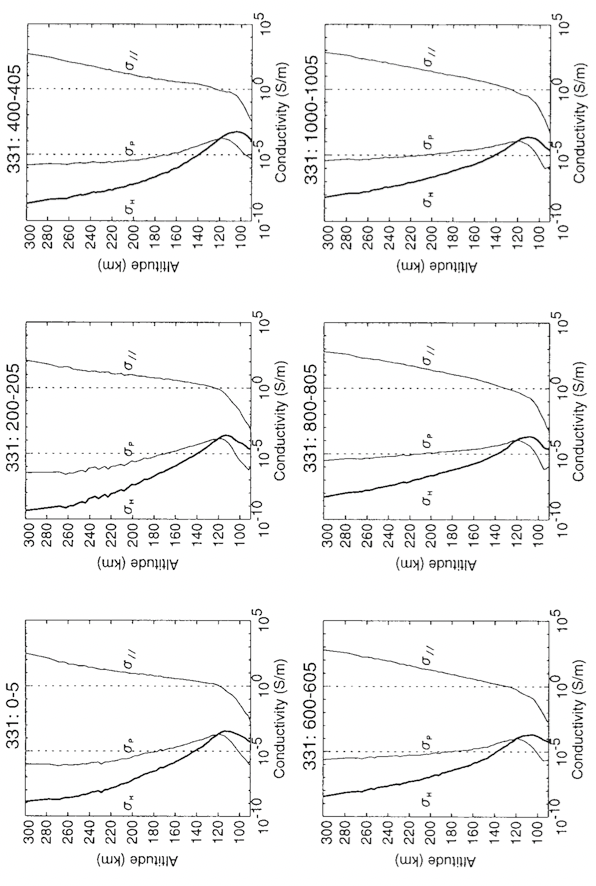
\includegraphics[width=.7\linewidth, angle=270]{bilder/L14_three_currents1.png}
        \caption{}\label{fig:L14_three_currents1}
    \end{subfigure}

    \begin{subfigure}[t]{.9\linewidth}
        \centering
        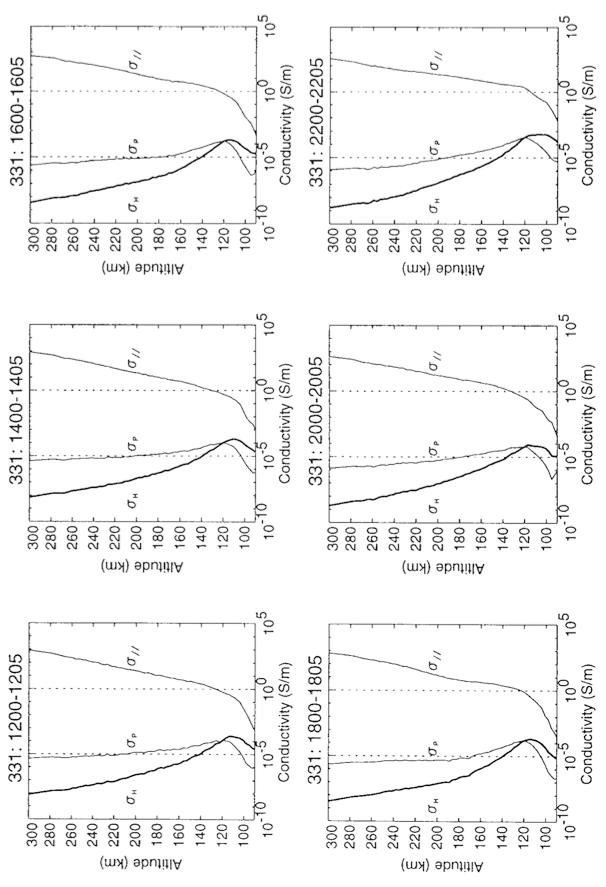
\includegraphics[width=.7\linewidth, angle=270]{bilder/L14_three_currents2.png}
        \caption{}\label{fig:L14_three_currents2}
    \end{subfigure}

    \caption{Examples of Pedersen, Hall, and parallel conductivity profiles (in siemens/m) as derived at the Tromsø auroral zone station for 12 different time intervals on March 31, 1992. (Courtesy Nozawa, 1995.)}\label{fig:L14_three_currents}
\end{figure}

\section{Height-dependent currents and heating rates}
We now look at the Joule heat dissipation rate. The height-dependent heat dissipation rate due to current flowing along an electric field perpendicular to \(\gf{B}\) (Joule heat dissipation) is given by
\begin{equation*}
    q_J(z)=\gf{j}(z)\cdot\gf{E}=(\sigma_P(z)\gf{E}_\perp-\sigma_H(z)\gf{E}_\perp\times\gf{B}/B)\cdot\gf{E}_\perp=\sigma_P(z)E_\perp^2
\end{equation*}
If we rewrite this in the neutral wind frame of reference, we get
\begin{equation*}
    q_J'(z)=\sigma_P(z)\gf{E'}_\perp^2=\sigma_P(z){\left(\gf{E}_\perp+\gf{u}_n(z)\times\gf{B}\right)}^2
\end{equation*}
We see that \(\sigma_H\) does not contribute to the heat dissipation. If \(\gf{E}_\perp+\gf{u}_n(z)\times\gf{B}=0\) then there are no Joule heating.

The magnitude of the current density at height \(z\) is
\begin{equation*}
    j{(z)}_\perp=\frac{e}{B}\frac{1}{\sqrt{1+k_i^2}}n_e(z)E_\perp'=\frac{e}{B}\frac{1}{\sqrt{1+k_i^2}}n_e(z)\left|\gf{E}_\perp+\gf{u}_n(z)\times\gf{B}\right|
\end{equation*}
The neutral wind is a very elusive parameter and extremely difficult to measure simultaneously at different altitudes for considerable lengths of time. This makes the neutral wind extra complicated to implement in models, and some averaging assumptions usually have to be made.

We can write up the Joule heating dissipation on another form, in the reference frame of the neutral wind, as
\begin{equation*}
    q_J'(z)=\gf{j}'(z)\cdot\gf{E}_\perp'(z)=\left(\sigma_P(z)\cdot\gf{E}_\perp'(z)-\sigma_H(z)\frac{\gf{E}_\perp'(z)\times\gf{B}}{B}\right)\cdot\gf{E}_\perp'(z)=\sigma(z){\left(\gf{E}_\perp'(z)\right)}^2\geq 0
\end{equation*}
or
\begin{equation*}
    q_J'(z)=\gf{j}'(z)\cdot\left(\gf{E}_\perp+\gf{u}_n(z)\times\gf{B}\right)=\gf{j}'(z)\cdot\gf{E}_\perp-\left(\gf{j}'(z)\times\gf{B}\right)\cdot\gf{u}_n(z)\geq 0
\end{equation*}

\section{Mapping of \(E\)-fields in the ionosphere}
We start by assuming finite conductivity \(\perp\gf{B}\Rightarrow \) electric field not necessarily conserved. Our coordinate system is defined by the vertical magnetic field being \(\gf{\widehat{B}}=-\f{z}\). The electric field is given by \(\gf{E}=E_x\f{x}+E_y\f{y}+E_z\f{z}\) and the current is given by \cref{eq:L14_current_equation} which we rewrite as
\begin{equation*}
    \gf{j}(z)=\left(\sigma_{P}E_x+\sigma_{H}E_y\right)\f{x}+\left(\sigma_{P}E_y-\sigma_{H}E_x\right)\f{y}+\sigma_{||}E_z\f{z}
\end{equation*}
This may be written up on tensor form as
\begin{equation*}
    \left(\begin{array}{c}
        j_x\\j_y\\j_z
    \end{array}\right)=\left(\begin{array}{ccc}
        \sigma_P & \sigma_H & 0\\
        -\sigma_H & \sigma_P & 0\\
        0 & 0 & \sigma_{||}
    \end{array}\right)\cdot
    \left(\begin{array}{c}
        E_x\\E_y\\E_z
    \end{array}\right)\Leftrightarrow\gf{j}=\widetilde{\sigma}\cdot\gf{E}
\end{equation*}

We now assume that conductivities are functions of \(z\) only. Since the current must be divergence free we find
\begin{equation*}
    \nabla\cdot\gf{j}=\sigma_P\p{x}{E_x}+\sigma_H\p{x}{E_y}+\sigma_P\p{y}{E_y}-\sigma_H\p{y}{E_x}+\p{z}{\left(\sigma_{||}E_z\right)}=0
\end{equation*}
Taking advantage of \(\nabla\times\gf{E}=0\) we write
\begin{equation*}
    \nabla\cdot\gf{j}=\sigma_P\left(\p{x}{E_x}+\p{y}{E_y}\right)+\p{z}{\left(\sigma_{||}E_z\right)}=0
\end{equation*}
Since the electric field must be deduced from a potential as \(\gf{E}=\nabla\phi \), we obtain
\begin{equation*}
    \p{xx}{\phi}+\p{yy}{\phi}+\frac{1}{\sigma_P}\p{z}{\left(\sigma_{||}\p{z}{\phi}\right)}=0
\end{equation*}
We will now introduce the following substitution
\begin{equation*}
    \tn{d}z'=\sqrt{\frac{\sigma_P}{\sigma_{||}}}\tn{d}z \Rightarrow \p{z}{}=\sqrt{\frac{\sigma_P}{\sigma_{||}}}\p{z'}{}
\end{equation*}
If we also introduce the geometric mean \(\sigma_m=\sqrt{\sigma_P\sigma_{||}}\) we get
\begin{equation*}
    \p{xx}{\phi}+\p{yy}{\phi}+\p{z'z'}{\phi}+\frac{1}{\sigma_m}\p{z'}{\sigma_m}\p{z'}{\phi}=0
\end{equation*}
If we now assume that \(\sigma_m=\sigma_0\exp(-z'/\alpha)\) this equation will be much simplified. \(\alpha \) is here a constant scale height. This does not limit the applicability of the solutions obtained since any reasonable conductivity profile can be closely approximated by a series of simple exponential functions. Inserting the new conductivity yields
\begin{equation*}
    \p{xx}{\phi}+\p{yy}{\phi}+\p{z'z'}{\phi}-\frac{1}{\alpha}\p{z'}{\phi}=0
\end{equation*}
where this can be solved by the method of separable variables. We will assume that the electrostatic potential is generated at a source level \(z_0'\) and that it has sinusoidal spatial variations with wavelength \(\lambda \) in both the \(x\)- and \(y\)-directions. The solution is then given by
\begin{equation*}
    \phi=\phi_0\exp\left[A\left(z'-z_0'\right)\right]\exp\left[\frac{2\pi i}{\lambda}\left(x+y\right)\right]
\end{equation*}
where \(A\) satisfies the equation
\begin{equation*}
    A^2-\frac{1}{\alpha}A-\frac{8\pi^2}{\lambda^2}=0
\end{equation*}
with roots
\begin{align*}
    A_1&=\frac{1}{2\alpha}-\sqrt{{\left(\frac{1}{2\alpha}\right)}^2+\frac{8\pi^2}{\lambda^2}}<0\\
    A_2&=\frac{1}{2\alpha}+\sqrt{{\left(\frac{1}{2\alpha}\right)}^2+\frac{8\pi^2}{\lambda^2}}>0
\end{align*}
Thus, the complete solution is
\coloredeq{eq:L14_electric_potential}{\phi=\left \{S_1\exp\left[A_1\left(z'-z_0'\right)\right]+S_2\exp\left[A_2\left(z'-z_0'\right)\right]\right \}\exp\left[\frac{2\pi{} i}{\lambda}\left(x+y\right)\right]\phi_0}
where \(S_1\) and \(S_2\) are constants to be determined by the boundary conditions of the problem. We see how the potential behave with regards to dampening at different heights in \cref{fig:L14_electric_potential}.
\begin{figure}[t]
    \centering
    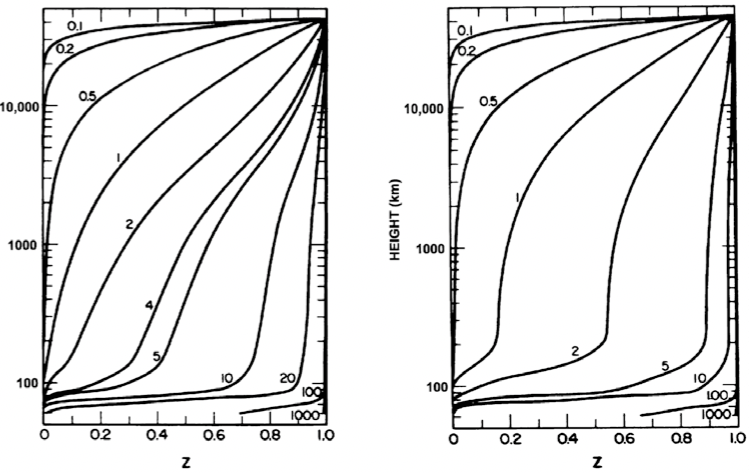
\includegraphics[width=.8\linewidth]{bilder/L14_electric_potential.png}
    \caption{(Left panel) The potential transmission factor (Z) as a function of altitude under daytime conditions. Z is the ratio between the potential at a particular altitude and at the source region. The labels on the curves refer to spatial wavelength (\(\lambda \)) in kilometers. (Right panel) The potential transmission factor (Z) as a function of altitude under night-time conditions. (From Reid, 1965.)}\label{fig:L14_electric_potential}
\end{figure}